To start off, let's analyze some filters that we can create with two elements.  The first of these will combine a resistor and a capacitor, as shown in Figure \ref{fig:RC_highpass}.

\begin{figure}
   \centering
%  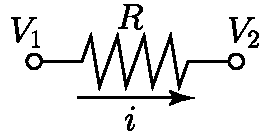
\includegraphics[width=0.5\linewidth]{figures/ohmsLaw}
  
\includegraphics{figures/toDo}
  \caption{A simple circuit composed of a source and two components.}
  \label{fig:RC_highpass}
\end{figure}
